\documentclass[11pt,a4paper]{article}
\usepackage[utf8]{inputenc}
\usepackage[T1]{fontenc}
\usepackage[spanish]{babel}
\usepackage{amsmath}
\usepackage{amssymb}
\usepackage{graphicx}
\usepackage{booktabs}
\usepackage{lmodern}
\usepackage{geometry}
\usepackage[hidelinks]{hyperref}
\geometry{margin=2.5cm}

\title{Planificación óptima de un evento}
\author{
Asignatura: Optimización I\\
Grado en Ciencia de Datos\\
Nieto Colás, Héctor; Mínguez Aguirre, Nicolás; Lara Domínguez, Unai\\
Aplicación web: \href{https://nicominguez-trabajo-opti-streamlit-app-bcagre.streamlit.app/}{\underline{streamlit}}\\
Curso académico: 2026/2027
}
\date{}

\begin{document}
\maketitle
\tableofcontents
\clearpage
\section{Contexto, datos y formulación --- Héctor Nieto Colás}

\subsection{Contexto}

Las Jornadas de Ciencia de Datos son un congreso de dos días dividido en ocho
franjas temporales: las franjas 1--4 corresponden al primer día y las 5--8 al
segundo. Se dispone de tres espacios: el Auditorio (200 plazas), el Aula de
ordenadores (40 plazas) y la Sala de seminarios (80 plazas).

La organización dispone de 18 actividades candidatas clasificadas en aprendizaje
automático, estadística e ingeniería de datos. Debe decidir qué actividades se
realizan y en qué espacio y franja comienza cada una. La decisión es real porque
no pueden programarse todas las actividades: el coste total asciende a 12.050
unidades, mientras que el presupuesto disponible es de 6.500.

El contexto aporta las siguientes condiciones:
\begin{itemize}
\item la conferencia inaugural y la de clausura son obligatorias;
\item los talleres y el \emph{hackathon} duran varias franjas y solo pueden
      celebrarse en el Aula de ordenadores;
\item las actividades con asistencia prevista superior a 80 personas no caben
      en la Sala de seminarios;
\item algunos ponentes invitados solo están disponibles en determinadas franjas;
\item existen actividades que compiten por el mismo público o ponente y no deben
      coincidir.
\end{itemize}

\subsection{Datos}

Los datos están separados del código en siete archivos CSV dentro de
\texttt{data/}, de forma que pueda resolverse cualquier otra instancia con el
mismo formato. Las estimaciones de costes, asistencias y valoraciones son los
valores definidos por el grupo para esta instancia.

\begin{table}[htbp]
\centering
\begin{tabular}{p{0.32\textwidth}p{0.58\textwidth}}
\toprule
Archivo & Contenido \\
\midrule
\texttt{actividades.csv} & Duración, categoría, asistencia, valoración,
coste y obligatoriedad \\
\texttt{espacios.csv} & Capacidad de cada espacio \\
\texttt{compat\_espacios.csv} & Espacios compatibles con cada actividad \\
\texttt{disp\_actividades.csv} & Franjas disponibles de cada actividad \\
\texttt{disp\_espacios.csv} & Franjas disponibles de cada espacio \\
\texttt{incompatibilidades.csv} & Pares de actividades incompatibles \\
\texttt{parametros.csv} & Presupuesto, pesos y horizonte temporal \\
\bottomrule
\end{tabular}
\caption{Archivos de datos de la instancia.}
\end{table}

El problema tiene una decisión real porque el coste total supera el presupuesto
y las duraciones suman 27 franjas, más que las 21 ocupaciones disponibles entre
los tres espacios en el horizonte considerado. La instancia contiene dos
actividades obligatorias, varias actividades de varias franjas, disponibilidad
temporal limitada y relaciones de incompatibilidad.

\subsection{Formulación}
\subsubsection{Conjuntos}
\begin{table}[H]
\centering
\begin{tabular}{p{0.20\textwidth}p{0.28\textwidth}p{0.42\textwidth}}
\toprule
\textbf{Símbolo} & \textbf{Definición} & \textbf{Significado} \\
\midrule
$I$ & $\{1,\ldots,18\}$ & Actividades candidatas. \\
$E$ & --- & Espacios disponibles. \\
$T$ & $\{1,\ldots,F\}$ & Franjas temporales. \\
$O$ & $O\subseteq I$ & Actividades obligatorias. \\
$P$ & --- & Pares $(i,j)$ de actividades incompatibles. \\
\bottomrule
\end{tabular}
\caption{Conjuntos del modelo.}
\end{table}

\subsubsection{Parámetros}
\begin{table}[H]
\centering
\begin{tabular}{p{0.20\textwidth}p{0.28\textwidth}p{0.42\textwidth}}
\toprule
\textbf{Símbolo} & \textbf{Definición} & \textbf{Significado} \\
\midrule
$d_i$ & --- & Duración de la actividad $i$, en franjas. \\
$a_i$ & --- & Asistencia esperada de la actividad $i$. \\
$v_i$ & --- & Valoración de la actividad $i$. \\
$c_i$ & --- & Coste de la actividad $i$. \\
$\mathrm{cap}_e$ & --- & Capacidad del espacio $e$. \\
$B$ & --- & Presupuesto máximo. \\
$\mathrm{comp}(i,e)$ & $\{0,1\}$ & Vale 1 si $i$ es compatible con $e$. \\
$\mathrm{dispA}(i,s)$ & $\{0,1\}$ & Vale 1 si $i$ puede celebrarse en $s$. \\
$\mathrm{dispE}(e,s)$ & $\{0,1\}$ & Vale 1 si $e$ está abierto en $s$. \\
$F$ & $8$ & Número de franjas. \\
$FD$ & $4$ & Número de franjas por día. \\
$\mathrm{dia}(t)$ & $\lceil t/FD\rceil$ & Día correspondiente a la franja $t$. \\
$w_A,w_V,w_N$ & $\geq 0$, suma 1 & Pesos de los tres criterios. \\
$N$ & $|I|$ & Número total de actividades candidatas. \\
$A_{\mathrm{tot}}$ & $\sum_{i\in I}a_i$ & Asistencia total de las actividades. \\
$V_{\mathrm{tot}}$ & $\sum_{i\in I}v_i$ & Valoración total de las actividades. \\
\bottomrule
\end{tabular}
\caption{Parámetros del modelo.}
\end{table}

\subsubsection{Variables}
\begin{table}[H]
\centering
\begin{tabular}{p{0.22\textwidth}p{0.20\textwidth}p{0.48\textwidth}}
\toprule
\textbf{Variable} & \textbf{Dominio} & \textbf{Interpretación} \\
\midrule
$x_{i,e,t}$ & $\{0,1\}$ & Vale 1 si la actividad $i$ comienza en el espacio
$e$ en la franja $t$, y 0 en otro caso. \\
$y_i$ & $\{0,1\}$ & Vale 1 si la actividad $i$ se programa, y 0 en otro caso. \\
\bottomrule
\end{tabular}
\caption{Variables binarias del modelo.}
\end{table}

\subsubsection{Función objetivo}
Se maximiza una suma ponderada de asistencia total, valoración total y número
de actividades programadas. La asistencia mide el alcance, la valoración mide
la calidad y el número de actividades evita una programación excesivamente
concentrada en pocas sesiones. Cada componente se normaliza para hacer
comparables sus unidades.

\[
\max Z=
\sum_{i\in I}y_i
\left(
w_A\frac{a_i}{A_{\mathrm{tot}}}
+
w_V\frac{v_i}{V_{\mathrm{tot}}}
+
w_N\frac{1}{N}
\right).
\]

Los pesos son no negativos y cumplen
$w_A+w_V+w_N=1$. Los valores por defecto son $(0.4,0.4,0.2)$; los escenarios
de análisis priorizan, respectivamente, la asistencia $(1,0,0)$, la valoración
$(0,1,0)$ y el número de actividades $(0.1,0.1,0.8)$.

\subsubsection{Restricciones}

\paragraph{R1. Selección única.}
Cada actividad se selecciona exactamente una vez o no se selecciona; por tanto,
no puede aparecer sin asignación ni ocupar varios espacios o franjas de inicio.
\[
y_i=\sum_{e\in E}\sum_{t\in T}x_{i,e,t}
\qquad\forall i\in I.
\]

\paragraph{R2. Actividades obligatorias.}
Las actividades marcadas como obligatorias deben formar parte de la
programación.
\[
y_i=1\qquad\forall i\in O.
\]

\paragraph{R3. Compatibilidad de espacio.}
Una actividad solo puede comenzar en espacios técnicamente compatibles con ella.
\[
x_{i,e,t}=0\qquad
\text{si }\mathrm{comp}(i,e)=0,
\qquad\forall i\in I,\ e\in E,\ t\in T.
\]

\paragraph{R4. Capacidad suficiente.}
La asistencia prevista no puede superar la capacidad del espacio asignado.
\[
x_{i,e,t}=0\qquad
\text{si }a_i>\mathrm{cap}_e,
\qquad\forall i\in I,\ e\in E,\ t\in T.
\]

\paragraph{R5. Disponibilidad de actividad y espacio.}
La disponibilidad se exige para todas las franjas ocupadas:
\[
x_{i,e,t}\leq
\mathrm{dispA}(i,s)\,\mathrm{dispE}(e,s),
\qquad
\forall i\in I,\ e\in E,\ t\in T,
s\in\{t,\ldots,t+d_i-1\}.
\]

\paragraph{R6. Horizonte y límite diario.}
\[
x_{i,e,t}=0
\quad\text{si}\quad
t+d_i-1>F
\quad\text{o}\quad
\mathrm{dia}(t)\neq\mathrm{dia}(t+d_i-1),
\qquad\forall i\in I,\ e\in E,\ t\in T.
\]

\paragraph{R7. Presupuesto.}
El coste total de las actividades seleccionadas no puede superar el presupuesto
disponible.
\[
\sum_{i\in I}c_i y_i\leq B.
\]

\paragraph{R8. Ocupación de un espacio.}
Una actividad que comienza en $t$ ocupa las franjas $t,\ldots,t+d_i-1$:
\[
\sum_{i\in I}
\sum_{t=\max(1,s-d_i+1)}^{s}
x_{i,e,t}
\leq 1
\qquad\forall e\in E,\;\forall s\in T.
\]

\subsubsection{Ampliación}

Como ampliación se incorporan incompatibilidades temporales mediante R9.
Dos actividades incompatibles pueden programarse, pero nunca simultáneamente,
aunque estén asignadas a espacios distintos. Los pares definidos son
$(3,10)$, $(12,16)$, $(9,17)$, $(7,18)$ y $(8,14)$.

La restricción representa actividades que compiten por público o ponente y
afecta tanto a la selección como a la asignación temporal. Por ejemplo, las
actividades 7 y 18 solo están disponibles en la franja 7 y no pueden
programarse conjuntamente.

\paragraph{R9. Incompatibilidad entre actividades.}
Las parejas incompatibles no pueden desarrollarse simultáneamente, aunque se
encuentren en espacios diferentes, para evitar competir por público o ponente.
Para cada par $(i,j)\in P$ y para cada franja $s\in T$:
\[
\sum_{e\in E}
\sum_{t=\max(1,s-d_i+1)}^{s}x_{i,e,t}
+
\sum_{e\in E}
\sum_{t=\max(1,s-d_j+1)}^{s}x_{j,e,t}
\leq 1.
\]


\clearpage
\section{Implementación, interfaz y documentación}

\subsection{Implementación}

\subsubsection{Carga y validación de datos}

La instancia se carga desde los siete archivos CSV de \texttt{data/}. La
implementación utiliza \texttt{pandas} para leer las tablas y
\texttt{PuLP} para construir el modelo entero. El archivo
\texttt{modelo.py}, dentro de \texttt{2\_implementacion/}, separa la carga y validación de los datos
de la construcción y resolución del modelo.

Antes de resolver se comprueban los encabezados obligatorios, los identificadores
duplicados, los valores numéricos y las relaciones entre actividades y espacios.
También se valida que el horizonte y las franjas por día formen un número entero
de días. Los errores de estructura o referencia se presentan como errores de
datos.

\subsubsection{Construcción y resolución}

La formulación se representa con variables binarias \texttt{y[i]} para la
selección y \texttt{x[i,e,t]} para la asignación inicial. Solo se crean variables
factibles desde el punto de vista de compatibilidad, capacidad, disponibilidad y
duración.

Las restricciones se aplican sobre cada franja: el presupuesto suma los costes
de las actividades seleccionadas y las actividades obligatorias toman el valor
uno. La ocupación impide solapes dentro de un espacio, también para actividades
de varias franjas. La ampliación impide que los pares incompatibles ocupen la
misma franja.

La función objetivo combina la asistencia, la valoración y el número de
actividades. La interfaz permite fijar los pesos de asistencia y valoración y
calcula \(w_N=1-w_A-w_V\), de modo que los pesos efectivos cumplen
\(w_A+w_V+w_N=1\). Como defensa adicional, el motor normaliza una terna recibida
desde código y rechaza una terna totalmente nula. El modelo se resuelve con el
solver HiGHS mediante \texttt{pulp.HiGHS}. La implementación distingue solución
óptima, problema inviable y error del solver o de los datos.

\subsection{Interfaz}

\subsubsection{Configuración y ejecución}

La interfaz se desarrolla con Streamlit en \texttt{streamlit\_app.py}. Permite
modificar el presupuesto y los pesos de asistencia y valoración. El peso del
número de actividades se calcula como \(w_N=1-w_A-w_V\), por lo que los tres
pesos siempre suman uno. La interfaz muestra además la terna efectiva y su suma.
Al pulsar el botón de resolución se indica si existe una solución óptima, si el
problema es inviable o si se ha producido un error.

\subsubsection{Presentación de resultados}

Para una solución óptima, la interfaz presenta el número de actividades,
asistencia, valoración, coste y presupuesto. También muestra un calendario
ordenado por espacios y franjas, identificado con etiquetas como \texttt{D1F3},
y una tabla con las actividades seleccionadas.

La tabla detallada conserva la actividad, categoría, duración, asistencia,
valoración, coste, espacio y franjas inicial y final. Permite comprobar la
asignación sin gráficos complejos. La interfaz carga la instancia principal
desde \texttt{data/} y ofrece la descarga CSV integrada de esta tabla de
actividades seleccionadas. Al mantener los archivos de entrada separados del
código, se puede modificar la instancia y ejecutar otra resolución compatible.

Las actividades no seleccionadas se muestran de forma compacta en una sección
plegable, para cumplir el requisito de informar de los descartes sin sobrecargar
la vista principal.

\begin{figure}[htbp]
\centering
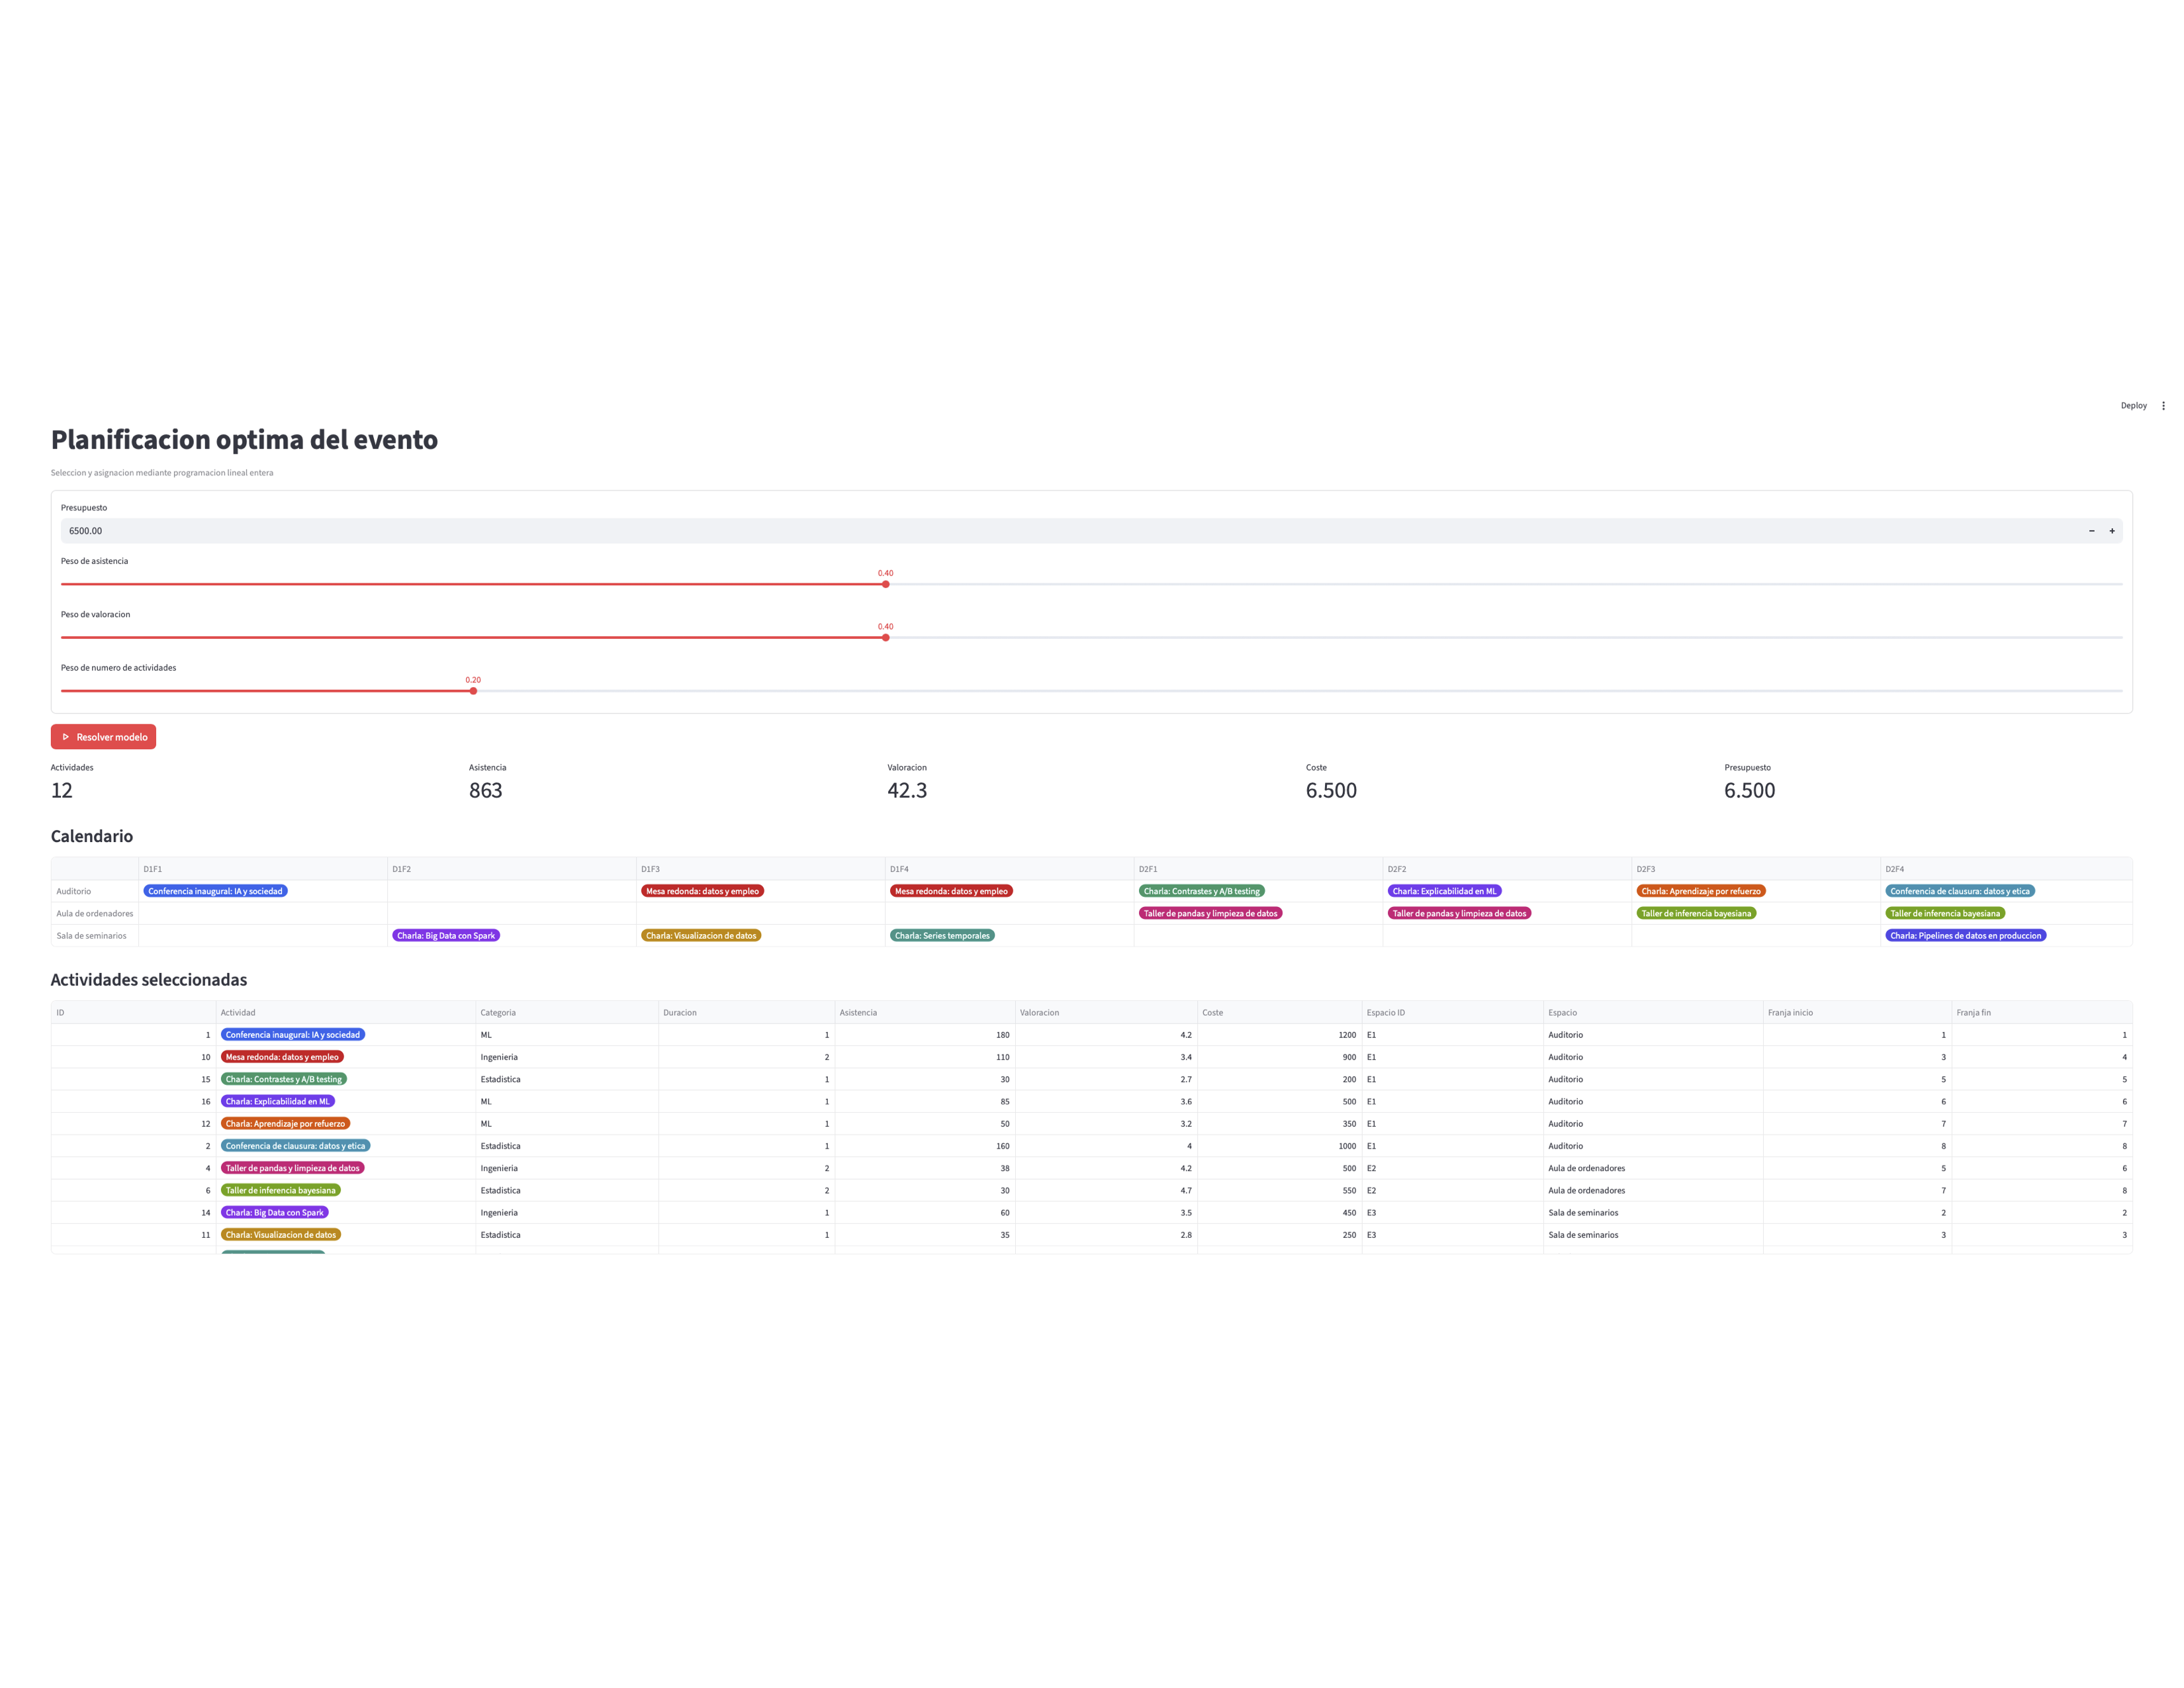
\includegraphics[width=\textwidth]{../images/ss.png}
\caption{Interfaz de Streamlit y resultados de una resolución.}
\label{fig:interfaz}
\end{figure}

\subsection{Documentación}

\subsubsection{Dependencias y ejecución}

Las dependencias se documentan en \texttt{requirements.txt} e incluyen
\texttt{streamlit}, \texttt{pandas}, \texttt{PuLP} y \texttt{highspy}. El
\texttt{README.md} indica la creación del entorno virtual, la instalación y la
ejecución local mediante \texttt{python -m streamlit run streamlit\_app.py}.

\clearpage
\section{Análisis, validación y conclusiones}

\subsection{Expectativas previas sobre el comportamiento del modelo}

Antes de proceder a la resolución numérica de la función objetivo, se analizan cualitativamente las expectativas teóricas para cada uno de los tres escenarios planteados, según las prioridades fijadas por la organización:

\begin{enumerate}
    \item \textbf{Escenario 1 - Priorización de Asistencia ($w_A = 1{,}0, w_V = 0{,}0, w_N = 0{,}0$):} 
    Se espera que el modelo seleccione las actividades de gran formato orientadas al Auditorio (E1) — como la \textit{Conferencia inaugural}, la de \textit{Clausura} o la \textit{Charla de IA generativa} — para maximizar el número total de asistentes. Esto ocurrirá a costa de descartar talleres específicos de menor aforo e inscribir un menor número total de actividades, debido al elevado coste de contratación de estos ponentes de gran alcance.

    \item \textbf{Escenario 2 - Priorización de Valoración ($w_V = 1{,}0, w_A = 0{,}0, w_N = 0{,}0$):} 
    Se anticipa una mayor concentración en talleres técnicos y prácticos de alta calidad percibida (como el \textit{Taller de redes neuronales} o el \textit{Hackathon de datos} en el Aula de Ordenadores E2). Aunque estas sesiones cuentan con un aforo máximo reducido (40 plazas), el modelo priorizará la excelencia cualitativa percibida sobre el volumen masivo de participantes.

    \item \textbf{Escenario 3 - Priorización del Número de Actividades ($w_N = 0{,}8, w_A = 0{,}1, w_V = 0{,}1$):} 
    Se espera una programación significativamente más densa, fundamentada en actividades de corta duración (1 franja horaria) y bajo coste económico. El objetivo prioritario en este caso es maximizar la ocupación de huecos del calendario disponible respetando el límite presupuestario de $6.500~\text{€}$.
\end{enumerate}

\begin{table}[htbp]
\centering
\caption{Tabla comparativa de indicadores clave por escenario ($B = 6.500~\text{€}$).}
\label{tab:comparativa_escenarios}
\renewcommand{\arraystretch}{1.3}
\setlength{\aboverulesep}{0pt}
\setlength{\belowrulesep}{0pt}
\resizebox{\textwidth}{!}{%
\begin{tabular}{|l c c c|}
\toprule
\textbf{Indicador Clave} & \textbf{Escenario 1 (Asistencia)} & \textbf{Escenario 2 (Valoración)} & \textbf{Escenario 3 (Nº Actividades)} \\
\midrule
\textbf{Pesos ($w_A / w_V / w_N$)} & $1{,}0 / 0{,}0 / 0{,}0$ & $0{,}0 / 1{,}0 / 0{,}0$ & $0{,}1 / 0{,}1 / 0{,}8$ \\
\textbf{Actividades programadas} & 10 & 12 & 12 \\
\textbf{Asistencia total esperada} & 880 personas & 788 personas & 863 personas \\
\textbf{Valoración total acumulada} & 33{,}6 puntos & 43{,}7 puntos & 42{,}3 puntos \\
\textbf{Presupuesto ejecutado} & 6.450~\text{€} & 6.500~\text{€} & 6.500~\text{€} \\
\bottomrule
\end{tabular}%
}
\end{table}

\subsection{Comentario razonado de compromisos (\textit{Trade-offs})}

A partir de la comparación cualitativa y cuantitativa de los resultados, se extraen los siguientes compromisos clave en la toma de decisiones:

\begin{itemize}
    \item \textbf{Tensión entre Asistencia y Valoración:} 
    La maximización de la asistencia (Escenario 1) concentra el presupuesto en ponencias de gran formato en el Auditorio (E1) con costes elevados y duraciones reducidas. Aunque se alcanza la asistencia máxima de $880$~asistentes, se dejan fuera talleres prácticos de menor aforo que aportan mayor satisfacción individual. En comparación directa con el Escenario 2, la estrategia masiva permite ganar $+92$~asistentes, pero a su vez implica la pérdida de $10{,}1$~puntos de valoración total acumulada y $2$~actividades en el programa.

    \item \textbf{Impacto del Criterio de Cantidad:} 
    El Escenario 3 alcanza un total de $12$~actividades programadas, igualando la cifra del Escenario 2. Sin embargo, al incorporar pequeñas ponderaciones para asistencia y valoración ($w_A = 0{,}1, w_V = 0{,}1$), logra un mejor equilibrio en el alcance de público ($863$ vs. $788$~asistentes) y mantiene una valoración elevada ($42{,}3$~puntos). Esto demuestra que el número de actividades por sí solo es un criterio menos discriminante que la calidad o el alcance si no se combina con pesos de equilibrio.
\end{itemize}

\subsection{Reproducibilidad técnica y pasos de ejecución}

Para garantizar la verificabilidad y reproducibilidad del trabajo desarrollado, la solución planteada se apoya en una arquitectura modular compuesta por un motor de optimización en \texttt{PuLP} y una interfaz interactiva en \texttt{Streamlit}.

El código fuente y las instancias de datos están alojados en un repositorio público de GitHub. La reconstrucción del entorno y la ejecución del modelo se realiza mediante los siguientes pasos:

\begin{enumerate}
    \item \textbf{Obtención del repositorio:} Clonar el proyecto o descargar la estructura de carpetas desde GitHub:
    \begin{verbatim}
    git clone https://github.com/nicominguez/trabajo_opti
    cd trabajo_opti
    \end{verbatim}
    
    \item \textbf{Creación del entorno e instalación de dependencias:} Se recomienda el uso de un entorno virtual para aislar las librerías necesarias:
    \begin{verbatim}
    python -m venv .venv
    source .venv/bin/activate  # En Windows: .venv\Scripts\activate
    pip install -r requirements.txt
    \end{verbatim}
    
    \item \textbf{Lanzamiento de la herramienta:}
    \begin{verbatim}
    streamlit run streamlit_app.py
    \end{verbatim}
\end{enumerate}

\subsection{Verificación de funcionalidades y control de inviabilidad}
Durante el proceso de validación del software se han verificado las siguientes características del sistema:

\begin{itemize}
    \item \textbf{Control dinámico de inviabilidad:} Ante configuraciones de parámetros con restricciones contradictorias (pesos ilógicos) o presupuestos insuficientes, el motor captura el estado devuelto por el solver (\texttt{Infeasible}) y la interfaz muestra una alerta explícita indicando que \textit{``no existe una programación valida con los parámetros actuales''}, evitando fallos de ejecución o salidas incoherentes.
    \item \textbf{Exportación de resultados:} Tras alcanzar la solución óptima, la aplicación permite descargar de forma directa dos archivos en formato CSV:
    \begin{enumerate}
        \item \texttt{calendario\_programacion.csv}: Matriz completa con la ocupación de los 3 espacios a lo largo de las 8 franjas horarias.
        \item \texttt{actividades\_seleccionadas.csv}: Resumen detallado de las actividades adjudicadas con sus costes, estimación de asistencia y valoración entre otros.
    \end{enumerate}
    \item \textbf{Consistencia de los indicadores:} Las ejecuciones directas del script y a través de la interfaz web arrojan resultados exactos a los tabulados en el análisis de escenarios del informe (880 asistentes en el Escenario 1 y 12 actividades en los Escenarios 2 y 3).
\end{itemize}

\subsection{Conclusiones}
La formulación de un modelo de programación lineal entera ha permitido automatizar la planificación del congreso de manera óptima, superando las limitaciones del diseño manual. El análisis comparativo demuestra la existencia de compromisos claros (\textit{trade-offs}) entre la cantidad masiva de público y la satisfacción cualitativa de los asistentes. La herramienta software desarrollada proporciona al equipo organizador un soporte cuantitativo riguroso para la toma de decisiones presupuestarias y logísticas.

\subsection{Declaración del uso de inteligencia artificial}

En cumplimiento de las directrices de transparencia en el uso de herramientas tecnológicas avanzadas, se declara que durante el desarrollo de este trabajo se ha contado con el apoyo de herramientas de Inteligencia Artificial Generativa (modelos de lenguaje / LLMs).

\subsubsection{Ámbitos de asistencia}
El uso de estas herramientas se ha limitado a las siguientes tareas de apoyo técnico y documental:
\begin{itemize}
    \item \textbf{Maquetación y formateo en \LaTeX:} Asistencia en la estructuración de ecuaciones matemáticas, tablas comparativas y organización general del documento fuente.
    \item \textbf{Depuración de código Python:} Apoyo en la revisión sintáctica y resolución de errores puntuales en los scripts del motor de optimización (\texttt{PuLP}) y de la interfaz gráfica (\texttt{Streamlit}).
    \item \textbf{Revisión estilística y lingüística:} Corrección ortotipográfica y refinamiento de la fluidez en la redacción de la memoria.
\end{itemize}

\subsubsection{Supervisión y autoría humana}
Los integrantes del grupo afirman y garantizan lo siguiente:
\begin{enumerate}
    \item \textbf{Diseño del problema y datos:} La contextualización del evento ("Jornadas de Ciencia de Datos"), la construcción de los 7 archivos CSV de datos y la formulación rigurosa del modelo matemático (conjuntos, parámetros, variables binarias y restricciones R1 a R9) son fruto del trabajo exclusivo del equipo.
    \item \textbf{Análisis e interpretación de resultados:} El planteamiento de las expectativas previas, la evaluación de los \textit{trade-offs} presupuestarios y las conclusiones han sido analizados y razonados críticamente por los miembros del grupo.
    \item \textbf{Validación de contenidos:} Todo código, formulación o texto desarrollado con asistencia de IA ha sido verificado, comprobado y validado técnicamente por los autores antes de su inclusión en el informe final.
\end{enumerate}

\clearpage
\section*{Anexo A. Datos de la instancia}
\addcontentsline{toc}{section}{Anexo A. Datos de la instancia}

\subsection*{A.1 Actividades}
Esta tabla describe las actividades candidatas, sus características, costes,
obligatoriedad, espacios compatibles y franjas disponibles.
\begin{table}[htbp]
\centering
\scriptsize
\resizebox{\textwidth}{!}{%
\begin{tabular}{rlccrrrrrl}
\toprule
Id & Actividad & Dur. & Categoría & Asist. & Valor. & Coste & Obl. & Esp. & Franjas \\
\midrule
1 & Conferencia inaugural: IA y sociedad & 1 & ML & 180 & 4.2 & 1200 & Sí & E1 & 1--2 \\
2 & Conferencia de clausura: datos y ética & 1 & Estadística & 160 & 4.0 & 1000 & Sí & E1 & 7--8 \\
3 & Taller de redes neuronales & 3 & ML & 35 & 4.8 & 900 & No & E2 & 1,2,3,5--8 \\
4 & Taller de pandas y limpieza de datos & 2 & Ingeniería & 38 & 4.2 & 500 & No & E2 & Todas \\
5 & Hackathon de datos & 3 & Ingeniería & 40 & 4.9 & 1100 & No & E2 & 5--8 \\
6 & Taller de inferencia bayesiana & 2 & Estadística & 30 & 4.7 & 550 & No & E2 & Todas \\
7 & Charla: IA generativa & 1 & ML & 190 & 3.6 & 1800 & No & E1 & 7 \\
8 & Charla: pipelines de datos en producción & 1 & Ingeniería & 45 & 3.0 & 350 & No & E1,E3 & Todas \\
9 & Charla: series temporales & 1 & Estadística & 40 & 3.0 & 250 & No & E1,E3 & 4 \\
10 & Mesa redonda: datos y empleo & 2 & Ingeniería & 110 & 3.4 & 900 & No & E1 & 2--4 \\
11 & Charla: visualización de datos & 1 & Estadística & 35 & 2.8 & 250 & No & E1,E3 & Todas \\
12 & Charla: aprendizaje por refuerzo & 1 & ML & 50 & 3.2 & 350 & No & E1,E3 & 6--8 \\
13 & Taller de SQL avanzado & 2 & Ingeniería & 30 & 4.0 & 400 & No & E2 & Todas \\
14 & Charla: Big Data con Spark & 1 & Ingeniería & 60 & 3.5 & 450 & No & E1,E3 & 1--4 \\
15 & Charla: contrastes y A/B testing & 1 & Estadística & 30 & 2.7 & 200 & No & E1,E3 & Todas \\
16 & Charla: explicabilidad en ML & 1 & ML & 85 & 3.6 & 500 & No & E1 & 6--8 \\
17 & Seminario de estadística espacial & 2 & Estadística & 45 & 3.0 & 350 & No & E1,E3 & 3--4 \\
18 & Charla: ética y sesgos algorítmicos & 1 & ML & 75 & 4.0 & 1000 & No & E1,E3 & 7 \\
\bottomrule
\end{tabular}%
}
\caption{Actividades de la instancia principal.}
\end{table}

\subsection*{A.2 Espacios y compatibilidades}
Esta tabla recoge los espacios disponibles, su capacidad y las franjas en las
que permanecen abiertos.
\begin{table}[htbp]
\centering
\begin{tabular}{llrl}
\toprule
Id & Espacio & Capacidad & Franjas abiertas \\
\midrule
E1 & Auditorio & 200 & 1--8 \\
E2 & Aula de ordenadores & 40 & 1,2,3,5--8 \\
E3 & Sala de seminarios & 80 & 2,3,4,6--8 \\
\bottomrule
\end{tabular}
\caption{Espacios de la instancia principal.}
\end{table}

Las compatibilidades se almacenan en \texttt{compat\_espacios.csv}. Además,
la compatibilidad de tipo debe combinarse con la capacidad: las actividades
7, 10 y 16 son compatibles con E3 por tipo, pero su asistencia supera las
80 plazas y no pueden asignarse a ese espacio.

\subsection*{A.3 Incompatibilidades y parámetros}
Esta tabla resume las parejas de actividades incompatibles y los parámetros
globales utilizados por el modelo.
\begin{table}[htbp]
\centering
\begin{tabular}{ll}
\toprule
Tipo & Valor \\
\midrule
Incompatibilidades & (3,10), (12,16), (9,17), (7,18), (8,14) \\
Presupuesto & 6500 \\
Pesos por defecto & $w_A=0.4$, $w_V=0.4$, $w_N=0.2$ \\
Franjas & 8; 4 franjas por día \\
\bottomrule
\end{tabular}
\caption{Parámetros globales e incompatibilidades.}
\end{table}

\clearpage
\section*{Anexo B. Contribución de cada integrante}
\addcontentsline{toc}{section}{Anexo B. Contribución de cada integrante}

La siguiente tabla resume las tareas realizadas por cada integrante a partir
del plan de trabajo de cada parte.

\begin{table}[htbp]
\centering
\renewcommand{\arraystretch}{1.2}
\begin{tabular}{p{0.22\textwidth}p{0.12\textwidth}p{0.56\textwidth}}
\toprule
\textbf{Integrante} & \textbf{Parte} & \textbf{Contribución} \\
\midrule
Héctor Nieto Colás & 1 &
\textbf{Objetivo:} definir el contexto, los datos y el modelo matemático que
selecciona, asigna y programa las actividades del evento.
\newline
\textbf{Asignaciones:} elegir y describir el contexto; presentar franjas,
espacios, actividades y restricciones naturales; caracterizar actividades y
espacios; aportar los valores y documentar los CSV externos; incluir las tablas
completas en el anexo; definir y justificar los tres criterios y sus pesos;
incorporar y justificar las incompatibilidades temporales; y definir conjuntos,
parámetros, variables, función objetivo y restricciones R1--R9. \\
\midrule
Nicolás Mínguez Aguirre & 2 &
\textbf{Objetivo:} convertir el modelo formulado en una implementación PLE
reproducible y una interfaz Streamlit mínima.
\newline
\textbf{Asignaciones:} cargar y validar los siete CSV; construir y resolver el
modelo binario con PuLP e HiGHS; devolver selección, asignación e indicadores;
distinguir solución óptima, inviabilidad y errores; implementar la interfaz,
sus controles, calendario, tablas y descarga CSV; incorporar la captura; y
documentar la ejecución de Streamlit y la compilación del informe. \\
\midrule
Unai Lara Domínguez & 3 &
\textbf{Objetivo:} redactar el análisis de los resultados y documentar el
software utilizado.
\newline
\textbf{Asignaciones:} redactar las expectativas de cada escenario; ejecutar
el modelo y tabular los indicadores; comentar los compromisos entre criterios;
documentar la reproducibilidad; verificar la gestión de inviabilidad, la
exportación CSV y la coincidencia entre interfaz e informe; incorporar la
captura; sintetizar el valor del modelo y los compromisos; y redactar la
declaración de inteligencia artificial y autoría humana. \\
\bottomrule
\end{tabular}
\caption{Contribución individual según los planes de trabajo de las tres partes.}
\end{table}


\end{document}
